\documentclass[a4paper, 12pt]{article}

\usepackage[T2A]{fontenc}
\usepackage[utf8]{inputenc}
\usepackage[english,russian]{babel}

\usepackage{wrapfig}
\usepackage{amsmath, amsfonts, amssymb, amsthm, mathtools}

\usepackage{pgfplots}
\pgfplotsset{compat=1.9}

\usepackage{graphicx}
\graphicspath{{pictures}}
\DeclareGraphicsExtensions{.pdf,.png,.jpg}

\author{\textbf{Муляревич Андрей Игоревич}}
\title{
\begin{LARGE}
\textbf{Лабораторная работа 1.4.1}\\
"Изучение экспериментальных погрешностей на примере физического маятника"
\end{LARGE}
}
\date{\today}

\begin{document}

\maketitle
\newpage

\textbf{Цель работы:} 1) на примере измерения периода свободных колебаний физического
маятника познакомиться с систематическими и случайными погрешностями, прямыми и косвенными измерениями; 2) проверить справедливость формулы для периода колебаний физического маятника и определить значение ускорения свободного падения; 3) убедиться в справедливости теоремы Гюйгенса об обратимости
точек опоры и центра качания маятника; 4) оценить погрешность прямых и косвенных измерений и конечного результата.

\textbf{Установка:} металлический стержень; опорная призма; торцевые
ключи; закреплённая на стене консоль; подставка с острой гранью для определения
цента масс маятника; секундомер; линейки металлические длиной 30, 50 и 100 см;
штангенциркуль; электронные весы; математический маятник (небольшой груз,
подвешенный на нитях).\\ Тонкий стальной стержень длиной {\large l} и массой {\large m}(точные
параметры определяются непосредственными измерениями) подвешивается на прикреплённой стене консоли с помощью небольшой призмы.
Призма острым основанием опирается на поверхность консоли. Острие ребра призмы образует ось качания маятника. Призму можно перемещать
вдоль стержня, изменяя положение точки подвеса (расстояние {\large a}). Период
колебаний измеряется непосредственно с помощью секундомера. Для проверки формулы (6) следует измерить зависимость колебаний {\large T} маятника
расстояния подвеса {\large a}. Расстояния измеряются линейками и штангенциркулем. Положение центра масс маятника может быть определено с помощью
балансирования маятника на вспомогательной подставке с острой гранью.


\textbf{Необходимая теория:}
\begin{enumerate}
\item Физический маятник -- маятник, рзамерами которого нельзя принебрегать. Для проведения экспиремента нам потребуется такие понятия как период колебаний, момент инерции. Момент инерции: $J = \sum_im_ir_i^2$, где $m_i$ масса рассматриваемой точки и $r_i$ расстояние от оси вращения до этой точки -- скалярная физическая величина, мера инертности во вращательном движении вокруг оси, подобно тому, как масса тела является мерой его инертности в поступательном движении.\\Момент инерции в центре массы для твердого стержня $J_c = \dfrac{ml^2}{12}$. Воспульзуясь теормемой Штейнера найдем момент инерции $J_a$ на расстоянии \textit{а} от центра масс до оси подвеса: $J_a = J_c + ma^2 = \dfrac{ml^2}{12} + ma^2$.
\item Воспользуемся законом Ньютона для вращательного движения $Fr = J_a\dfrac{d\omega}{dt}$ и получим после подстановки $J_a$ и $F = mg$
\[J_a\dfrac{d\omega}{dt} = -mga\sin \varphi \approx -mga\varphi\]
После преобразований:
\[J_a\ddot{\varphi}+mga\varphi=0\]
\begin{minipage}{\linewidth}
\begin{wrapfigure}{r}{4cm}
\begin{center}
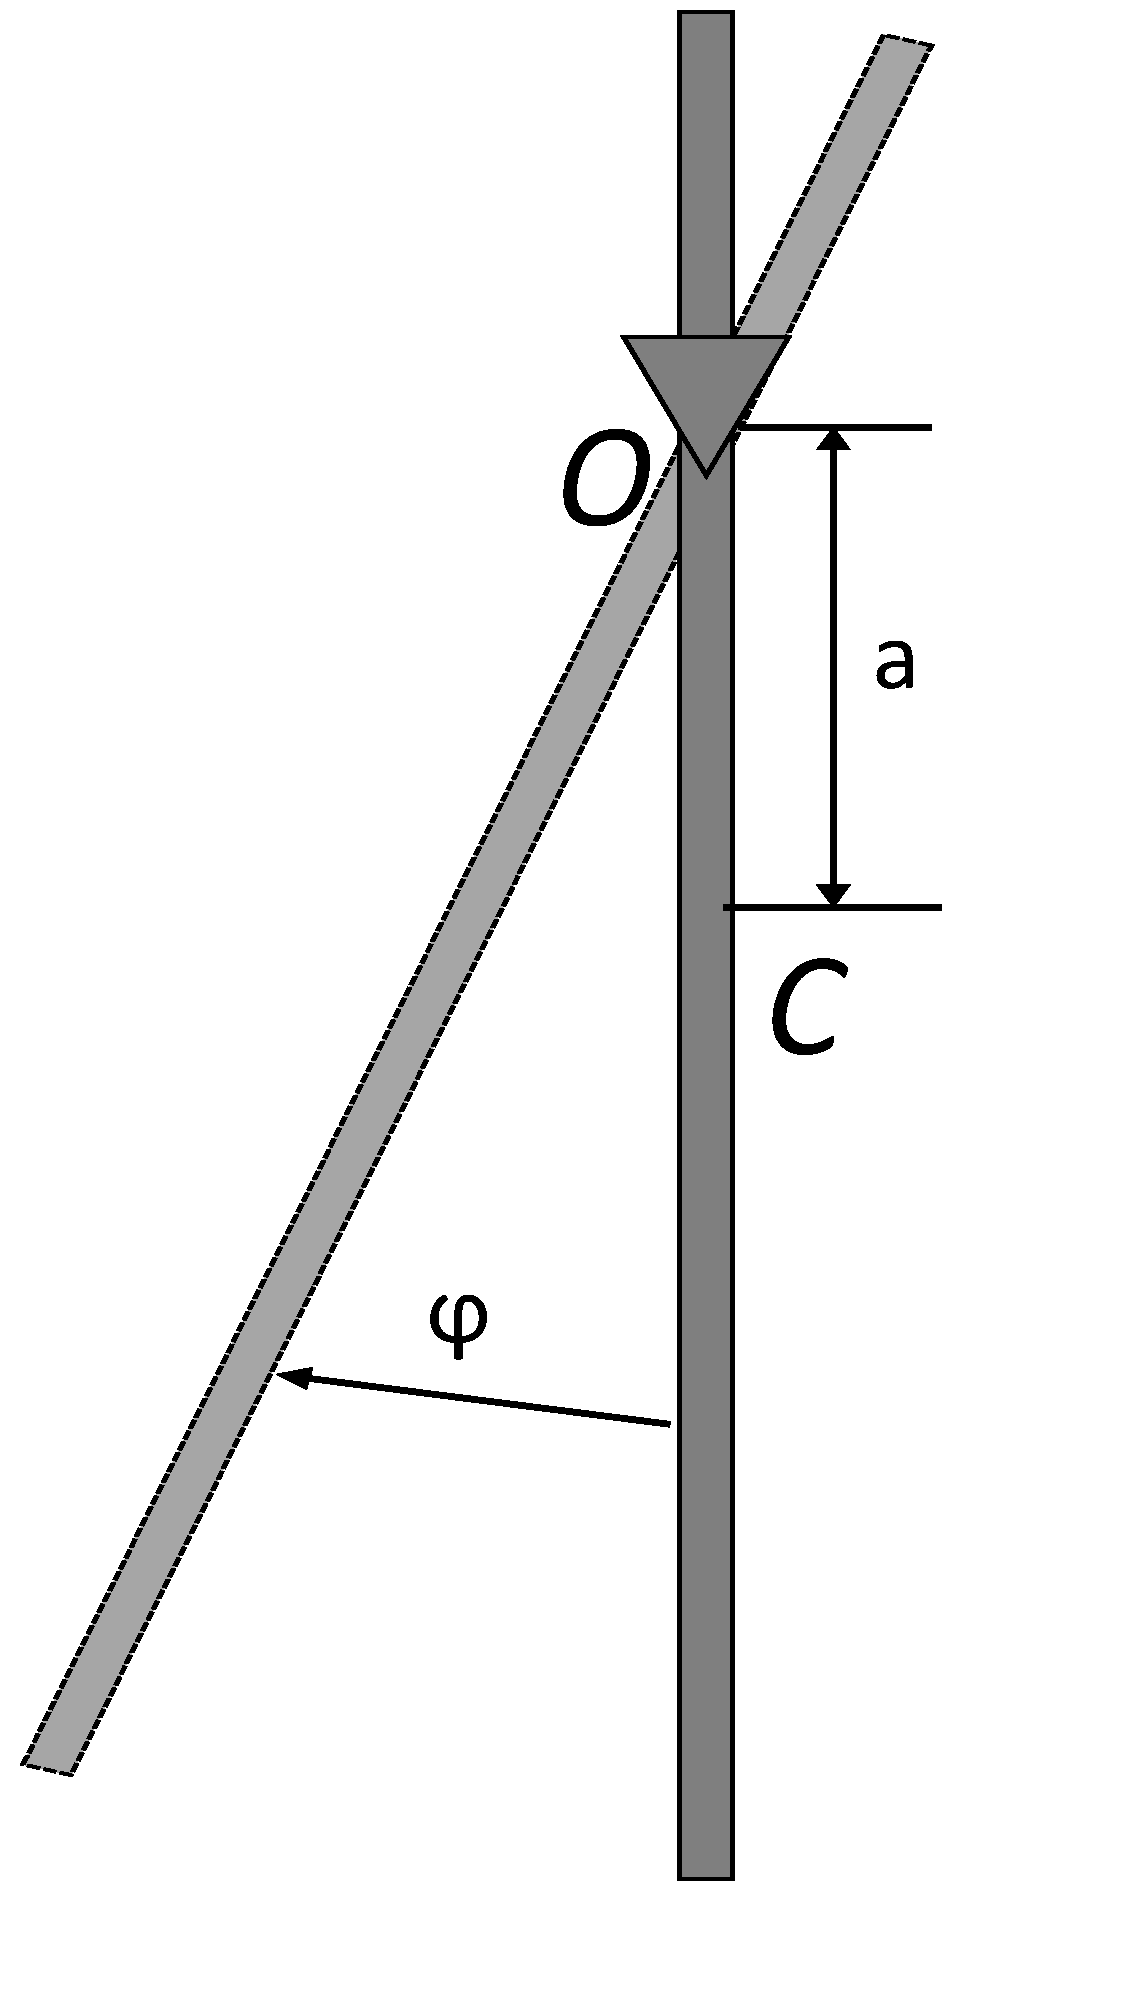
\includegraphics[width=4cm]{ustanovka}
\end{center}
\caption{Стержень как физичексий маятник}
\end{wrapfigure} Из полученнможно сделать вывод,
что при малых амплитудах отклонения движение свободного физического маятника будет иметь характер \textit{гармонических колебаний}, аналогично колебаниям груза на пружине или математического маятника.  Решением
данного дифференциального уравнения являются гармонические колебания, описываемые законом:
\[ \varphi(t) = A\sin (\Omega t + \alpha)\]
где $\Omega = \dfrac{2\pi}{T} = \sqrt{\dfrac{mga}{J_a}}$ -- угловая частота колебаний, $A$ -- амплитуда колебаний, $\alpha$ -- начальная фаза колебаний. Амплитуда и фаза колебаний определяются начальными условиями. При этом угловая частота (и период) малых колебаний не зависит ни от фазы, ни от амплитуды. Однако при достаточно больших амплитудах последнее утверждение нарушается. Оно справедливо в той мере, в которой справедливо приближение $\sin \varphi \approx  \varphi$, сделанное нами при выводе.
\end{minipage}
\item Предыдущие законы записаны для случая идеального маятника в отсутствие затухания. Реальный маятник подвержен, в частности, сопротивлению воздуха, а также трению в оси подвеса, что приводит к постепенному затуханию его колебаний. Если трение не слишком велико, колебания маятника всё ещё могут быть описаны формулой для горманических колебаний, но амплитуду колебаний следует считать медленно убывающей функцией времени: $A(t)$. Относительную убыли амплитуды за одно колебание $ \gamma= \dfrac{\vert\Delta A\vert}{A} $ называют декрементом затухания. Величина $\gamma$ является характеристикой всех потерь энергии в колебательной системе. Как правило, $\gamma$ можно считать постоянной, и тогда
интегрируя уравнение $ -\gamma= \dfrac{\Delta A}{A} $, получаем:
\[A(t) = A_0e^{-\gamma t}\]
Таким образом, величина $\tau_{\text{зат}} = 1\diagup \gamma $ -- это время, за которое амплитуда колебаний падает в $e$ раз. Оно может быть легко измерено экспериментально. Затухание можно считать малым, если это время велико по сравнению с временем одного колебания: $\tau_{\text{зат}} >> T$.
\item Определим так называемую \textit{приведённую длину} физического маятника:
\[l_{\text{пр}} = a + \dfrac{l^2}{12a}\]
Смысл этой длины в том, что физический маятник длиной $l$, подвешенный в точке $a$, имеет тот же период малых колебаний, что и математический маятник длиной $l_{\text{пр}}$.\\
С понятием «приведённой длины» связана теорема Гюйгенса.
\item В нашем экспиременте физическим маятником является стержень совместно с призмой, поэтому требуется учесть влияние призмы на период колебаний.На практике учесть влияние призмы можно следующим образом.\\
Период колебаний такого маятника:
\[T = \sqrt{\dfrac{J_{\text{пр}} + J_{\text{ст}}}{m_{\text{пр}}ga_{\text{пр}} + m_{\text{ст}}ga_{\text{ст}}}}\]
Поскольку расстояние $a_{\text{пр}}$ от оси до центра масс призмы сложно поддается расчету то можно исключить его, измеряя положение центра
масс всей системы. Пусть $x_c$ -- расстояние от оси подвеса до центра масс системы, тогдп по определению имеем:
\[x_c = \dfrac{m_{\text{пр}}a_{\text{пр}} + m_{\text{ст}}a_{\text{ст}}}{m_{\text{пр}} + m_{\text{ст}}}\]
Тогда можно изменить формулу для периода колебаний:
\[T = 2\pi\sqrt{\dfrac{\dfrac{l^2}{12} + a^2}{g\beta x_c}}\]
где $\beta = 1 + \dfrac{m_{\text{пр}}}{m_{\text{ст}}}$.\\
Таким образом, для более точного измерения g следует для каждого положения призмы измерять величины $a$ (положение призмы относительно
центра масс стержня), $x_c$ (положение центра масс стержня с призмой относительно оси вращения) и период соответствующих малых колебаний.
\item \textbf{Расчет погрешностей:}
\begin{enumerate}
\item \textbf{Расчет погрешностей прямых измерений:}\\
Формулы для расчета:
\[x_{\text{ср}} = \frac{1}{N} \sum_i^N x_i\]
\[\sigma_{\text{отд}} = \sqrt{\dfrac{1}{N-1}\sum_i^N(x_i - x_{\text{ср}})^2} \]
\[\sigma_{\text{ср}} = \dfrac{\sigma_{\text{отд}}}{\sqrt{N}} = \sqrt{\dfrac{1}{N(N-1)}\sum_i^N(x_i - x_{\text{ср}})^2}\]
, где $x$ -- значение измеряемой велечины, в пределах $\pm\sigma_{\text{отд}}$  от $x_{\text{ср}}$ вероятность измерения равна 68\%.\\
Случайная асболютная и относительная погрешность измеряемой величины:
$\sigma_{\text{сл}} = \sigma_{\text{ср}}$, $\varepsilon_{\text{сл}} =
\dfrac{\sigma_{\text{сл}}}{x_{\text{ср}}}$\\
Систематическая погрешность приборов можно узнать из паспорта прибора, либо она может быть указана на самом приборе, если ее величина неизвестна то стоит положить что $\sigma_{\text{сист}}$ равна половине цены деления прибора.\\
Полная погрешность измеряемой величины равна:
\[\sigma_{\text{полн}} = \sqrt{\sigma_{\text{сл}}^2 + \sigma_{\text{сист}}^2}\]
\item \textbf{Расчет погрешностей косвенных измерений по МНК (метод наименьших квадратов):}\\
Если известно что $y(x) = xa+b$, а также известны некторое кол-во точек на графике с координатами $x$ и $y$, можно оценить погрешнотси константных величин $a$ и $b$, для этого нужно воспользоваться формулами:
\[ a = \dfrac{\langle xy\rangle - \langle x\rangle \langle y\rangle}{\langle x^2\rangle - \langle x\rangle ^2}\]
\[b = \langle y\rangle - \langle x\rangle a\]
\[\sigma_a = \frac{1}{\sqrt{N}}\sqrt{\dfrac{\langle y^2\rangle - \langle y \rangle ^2}{\langle x^2\rangle - \langle x\rangle ^2} - a^2}\]
\[\sigma_b = \sigma_a\sqrt{\langle x^2\rangle - \langle x\rangle ^2}\]
\end{enumerate}
\end{enumerate}

%%%%%%%%%%%%%%%%%%%%%%%%%%%%%%%%%%%%%%%%%%%%%%%%%%%%%%%%%%%%%%%%%%%%%%%%

\textbf{Ход работы:}
\begin{enumerate}
\item Знакомимся с используемыми в работе измерительными приборами: линейками, весами, секундомером. Определяем максимальную систематическую погрешность каждого из них (абсолютное и относительное значение: $\varepsilon_{\text{лин}}^{\text{сист}} = 0,05\% $ , $\sigma_{\text{лин}}^{\text{сист}} = 0,5 \text{мм}$ ,$\varepsilon_{\text{вес}}^{\text{сист}} = \dfrac{\sigma_{\text{вес}}^{\text{сист}}}{m_{\text{пр}}} = 0,01\% $ , $\sigma_{\text{вес}}^{\text{сист}} = 0,05\text{г}$ , $\varepsilon_{\text{сек}}^{\text{сист}} = 0,1\% $ , $\sigma_{\text{сек}}^{\text{сист}} = 0,1c$. Оцениваем максимальную погрешность , с которой имеет смысл измерять период колебаний маятника по формуле:
\[\varepsilon_{\text{макс}} = \sqrt{\varepsilon_{\text{лин}}^2 + \varepsilon_{\text{штан}}^2 + \varepsilon_{\text{сек}}^2} =  0,12 \%\] 
\item Измеряем длину стержня $l$. Взвешиваем штангу и призму на электронных весах. Оцениваем погрешности измерений (абсолютные и относительные значения): 
$l = 1000 \pm 0,5 \text{мм}$, $\varepsilon_l = 0,05\%$, $m_{\text{ст}} = 871,1\pm 0,5 \text{г}$, $\varepsilon_{m_{\text{ст}}} = 0,05\%$, $m_{\text{пр}} = 69,2\pm 0,05\text{г}$, $\varepsilon_{m_{\text{пр}}} = 0,07\%$. Рассчитываем значение множителя $\beta$: $\beta = 1,08$.
\item Снимаем со стержня призму и с помощью подставки определяем положение центра масс стержня. Устанвливаем призму на расстоянии $ a = l / 4$ от центра стержня, измеряем точное положение $a$ острия призмы относительно центра стержня. Измеряем положение центра масс конструкции $x_c$, сбалансировав маятник с призмой на острие вспомогательной подставки. Оценвем погрешности измерения расстояний $a$ и $x_c$: $a = 25,00 \pm 0,05 \text{мм}$, $\varepsilon_a = 0,2\%$, $x_c = 23,00 \pm 0,05\text{м}^{-2}$, $\varepsilon_{x_c} = 0,1\%$.
\item Проводим первый предварительный опыт по измерению периода колебаний. 
\begin{enumerate}
\item Устанавливаем маятник на консоли и отклоняем его на малый
угол (не более $5^{\circ}$). Убеждаемся, что он качается без помех, призма
не проскальзывает, и колебания затухают слабо.
\item Измеряем время $n = 10$ полных колебаний маятника.
\item Вычисляем период колебаний $T = t/n$ и расчитываем предварительное значение $g$. Проверяем, что оно отличается
от табличного не более, чем на $10\%$.
\[ T = \dfrac{t}{N} = 1,541 \text{с} \]
\[ g = 9,76 \dfrac{\text{м}}{\text{с}^2}\]
\end{enumerate}
\item Проведим серию измерений для экспериментального определения случайной погрешности измерения времени с помощью секундомера (эта погрешность связана с такими случайными факторами, как время реакции экспериментатора, случайные колебания воздуха и т.п.).$\sigma_T = \text{с}$.
\begin{enumerate}
\item Повторяем измерение периода $n = 10$ колебаний 8–10 раз, каждый раз останавливая и заново отклоняя маятник примерно на
один и тот же малый угол; результаты занесим в таблицу
\begin{minipage}{\linewidth}
\begin{wrapfigure}{r}{4cm}
\begin{tabular}{|c|c|}
\hline 
№ опыта & t, с \\ 
\hline 
1 & 15,34 \\ 
\hline 
2 & 15,06 \\ 
\hline 
3 & 15,19 \\ 
\hline 
4 & 15,31 \\ 
\hline 
5 & 15,25 \\ 
\hline 
6 & 15,35 \\ 
\hline 
7 & 15,30 \\ 
\hline 
8 & 15,22 \\ 
\hline 
9 & 15,41 \\ 
\hline \hline
$t_{\text{ср}}$ & 15,28 \\ 
\hline 
$\sigma_{\text{t}}^{\text{сист}}$ & 0,103\\ 
\hline 
$\sigma_{\text{t}}^{\text{сл}}$ & 0,015\\ 
\hline 
$\sigma_{\text{t}}^{\text{полн}}$ & 0,104\\ 
\hline 
\end{tabular} 
\end{wrapfigure}
\item Вычисляем среднее значение полученных результатов $t_{\text{ср}}$, а также определяем случайную погрешность измерения времени как среднеквадратичное отклонение полученных результатов: $\sigma_{\text{t}}^{\text{сл}}$.
\item Определеям инструментальную (систематическую) погрешность используемого секундомера $\sigma_{\text{t}}^{\text{сист}}$, и вычисляем полную погрешность $\sigma_{\text{t}}^{\text{полн}}$. Заносим данные в таблицу справа.
\end{minipage}\\\\\\\\\\\\\
\end{enumerate}
\item Используя погрешность измерения времени из предыдущего пункта,
оцените число колебаний $n$, по которому следует измерять период,
чтобы относительная погрешность измерений периода соответствовала точности измерений $\varepsilon_{\text{макс}}$, , оценённой в п. 1.
\[ n = \dfrac{\sigma_{\text{t}}^{\text{полн}}}{T_{\text{ср}}\varepsilon_{\text{макс}}} \approx 60\]
\item Поместите призму в другое положение, измерьте её положение $a$ относительно центра, положение центра масс системы $x_c$ и время $n$ полных
колебаний, где значение $n$ выбрано в п. 6. Проведите измерения периода для 10–12 значений $a$. Для каждого измерения рассчитайте значения $g$, Занесите результаты в таблицу.
\begin{tabular}{|c|c|c|c|c|c|c|}
\hline 
№ опыта & $a$,  $\text{см}$ & $x_c$, $\text{см}$ & $n$ & $t_n$, $\text{с}$ & $T$, $\text{с}$ & $g$, $\text{м/с}^2$ \\ 
\hline 
1 & 40 & 36,5 & 60 & 93 & 1,55 & 9.96 \\ 
\hline 
2 & 30 & 27,5 & 60 & 91 & 1,52 & 9.97 \\ 
\hline 
3 & 25 & 23 & 60 & 90 & 1,5 & 10.30 \\ 
\hline 
4 & 20 & 18,5 & 60 & 97 & 1,61 & 9.4 \\ 
\hline 
5 & 15 & 14 & 60 & 98 & 1,63 & 10.4 \\ 
\hline 
6 & 10 & 9,5 & 60 & 133 & 2,22 & 7.29 \\ 
\hline
\end{tabular} \\\
\item Проведем опыт по определению приведённой длины маятника:
\begin{enumerate}
\item для одного значения $a = 40 \text{ см}$ вычислим приведённую длину физического мятника.\\ $l_{\text{пр}} = 60,8 \text{ cм}$;
\item установим соответствующую длину математического маятника и
проверем равенство периодов колебаний физического и математического маятников (с учётом погрешностей измерений):
\[ T_{\text{мм}} = 2\pi \sqrt{\dfrac{l_{\text{пр}}}{g}} = 1,54\text{ с}\approx T_{\text{фм}} = 1,528\text{ с}\]
\item поместим призму в центр качания и перевернём маятник; убедимся, что период колебаний не изменился в пределах погрешности.
\end{enumerate}
\textbf{Обработка результатов измерений}
\item Усредним значения ускорения свободного падения $g$, полученные в
п. 7. Оценим погрешность результата.
\[ g_{\text{ср}} = 9,56 \pm 0,47\dfrac{\text{м}}{\text{с}^2}, \sigma_g = 0,47 \dfrac{\text{м}}{\text{с}^2}, \varepsilon_g = 4,9\%\]
\item Постройте график зависимости периода колебаний $T$ от $a$. Убедитесь, что зависимость $T(a)$ имеет минимум; определите по графику положение минимума $T_{min} = \text{с}$.
\newpage
\begin{tikzpicture}
\begin{axis}[
	height = 0.3\paperheight, 
	width = 0.6\paperwidth,	
	axis x line = bottom,
	axis y line = left,
	ymin = 1.4, ymax = 2.4,
	xmin = 0,
	title = График зависимости $T(c)$ ,
	xlabel = {a, $\text{м}$},
	ylabel = {T, $\text{с}$}
	]
	\addplot+ [smooth,] 
		coordinates 
		{
		(40, 1.55) (30, 1.52) (25, 1.5) (20, 1.61) (15, 1.64) (10, 2.22)
		};
\end{axis}
\end{tikzpicture}\\\
\[T_{\text{мин}} = 1,5 \text{ с}\]
\item Построим график, откладывая по оси абсцисс величину $u = T^2x_c$, , а по оси ординат величину $v = a^2$. Согласно формуле \
\[T = 2\pi\sqrt{\dfrac{\dfrac{l^2}{12} + a^2}{g\beta x_c}}\]
, этот график должен иметь вид прямой линии — убедимся в этом.
\newpage
\begin{tikzpicture}
\begin{axis}
[
	height = 0.3\paperheight, 
	width = 0.6\paperwidth,	
	axis x line = bottom,
	axis y line = left,
	ymin = 20, ymax = 100,
	xmin = 0,
	title = График зависимости $v(u)$ ,
	xlabel = {$v$, $\text{см}^2$},
	ylabel = {$u$, $\text{см} \cdot \text{с}^2$}
]
\addplot+[blue, only marks, mark size = 3 pt,] 
	coordinates
	{
		(1600, 87.69) (900, 63.54) (625, 51.75) (400, 47.95) (225, 39.2) 
		(100, 43.8) 	
	};
\addplot [
	blue,
	domain = 50:1600,		
	]
	{0.0312*x + 35.8};
\end{axis}
\end{tikzpicture}\\

Коэфициент корелляции $r = 0,96$.
\item Методом наименьших квадратов определим параметры $(k,b)$ наилучшей прямой $u = kv + b$ и их погрешности ($\sigma_k$ и $\sigma_b$). По наклону прямой, используя формулу 
\[T = 2\pi\sqrt{\dfrac{\dfrac{l^2}{12} + a^2}{g\beta x_c}}\]
, рассчитаем величину ускорения свободного падения $g$.
\[ k = 0,0371 ; \sigma_k = 0,0008; b = 35,8 ; \sigma_b = 1,9\] 
\[ k = \dfrac{4\pi^2}{\beta g} \Rightarrow g = \dfrac{4\pi^2}{\beta k} = 9,85 \dfrac{\text{м}}{\text{с}^2}\]
\item Оценим погрешность измерения величины $g$ в п. 12. Учтём, что погрешность может включать как случайную составляющую (определяемую по методу наименьших квадратов), так и систематическую (погрешность величин $T^2x_c$ и $a^2$).Сравним результат расчёта по п. 13 с
непосредственным усреднением, проведённым в п. 9.
\[\sigma_u = 2T_{\text{ср}}x_c\sigma_T = 5,61\text{см} \cdot \text{с}^2; \sigma_v = 2\langle a\rangle\sigma_a = 2,5 \text{см}^2\]
\[\varepsilon_u = \dfrac{\sigma_u}{T_{\text{ср}}^2x_c} = \dfrac{2\sigma_T}{T_{\text{ср}}} = 0,02; \varepsilon_v = \dfrac{2\sigma_a}{\langle a\rangle} = 0,03; \varepsilon_k = \dfrac{\sigma_k}{k} = 0,02\]
\[\varepsilon_g^{'} = \sqrt{\varepsilon_k^2 + \varepsilon_u^2 + \varepsilon_v^2} = 0,041 = 4,1\%\]
\[ g = 9,85 \pm 0,41 \dfrac{\text{м}}{\text{с}^2}\]
\end{enumerate}
\textbf{\large Вывод:}
На примере измерения периоды свободных колебаний физического маятника познаколмился с систематическими и случайными погрешностями, прямыми и косвенными измерениями. Проверил справедливость формулы периода свободных колебаний для физического маятника из которых определил экспериментальное значение ускорения свободного падения на широте Москвы $g = 9,85 \dfrac{\text{м}}{\text{с}^2}$ из косвенных измерений по МНК и $g = 9,56 \dfrac{\text{м}}{\text{с}^2}$ из прямых измерений. Точное значение ускорения свободного падения на широте Москвы $g \approx 9,8152 \approx 9,8 \dfrac{\text{м}}{\text{с}^2}$ (источник Википедия). Разницы экспирементальных и точного занчения $g$ равна 0,5\% и 2,4\% для $g$ по МНК и из прямых измерениям соответсвенно. Относительные погрешности соответсвенно равны $\varepsilon_g = 4,1\%$ и $\varepsilon_g^{'} = 4,9\%$ $\Rightarrow$ значение $g$, расчитанное по МНК точнее чем расчитанная из прямых измерений по формуле периода колебаний для физ. маятника. 
Убедился в справедливости теоремы Гюйгенса об обратимости точек опоры и центра качания.  
\end{document}